%%
%%  AaltoTheses - LaTeX-tutkielmapohjat Aalto-tyylille
%%
%%  Hannu Tiitu
%%  hannu@tiitu.fi
%%
\begin{filecontents*}{\jobname.xmpdata}
  \Title{Digital Twins in Cloud Native applications}
  \Author{Hung Vu}
  \Keywords{digital twin\sep cloud native\sep software development\sep artificial intelligence\sep distributed systems\sep software development \sep CI-CD}
  \Publisher{Aalto University}
\end{filecontents*}
\documentclass[oneside,pdfa]{aaltoseries}
\makeatletter
\@ifpackageloaded{inputenc}{%
  \inputencoding{utf8}}{%
  \usepackage[utf8]{inputenc}}
\hypersetup{hidelinks}              
\makeatother
\usepackage[finnish,english]{babel}   
\usepackage{setspace}                 % Rivivälin säätämiseksi
\usepackage{afterpage}                % Sivun taustaväri
\microtypesetup{letterspace=25}       % Kannen harvaan välistykseen
\usepackage{xcolor, soul}

% Custom commands

\newcommand{\parendline}[1]{\paragraph{#1}~\\}


% Bibiography
\bibliographystyle{ieeetran}




\author{Hung Vu}
\title{Digital Twins Technology in Cloud Native Applications: Challenges, Best Practices, and Future Potential}

\begin{document}



%%  KANSI  ---------------------------------------------

\thispagestyle{empty}
\setcounter{page}{0}  % Kansisivulle sivunumero 0

% Kansisivun marginaalit
\newgeometry{left=23.2mm,right=23.2mm,top=13.5mm,bottom=18mm}

% Punainen kansisivu
\pagecolor{aaltoRed}\afterpage{\nopagecolor}
{\color{black}  % Musta teksti

{\parindent0pt % Kappaleiden sisennys pois päältä
{\fontsize{11.9pt}{11.9pt}\bfseries\sffamily\lsstyle Bachelor’s Programme in Science and Technology}

\color{white}  % Valkoinen teksti alkaa

\vspace{13.1mm}

\begin{spacing}{3.1}
{\fontsize{35}{35}\selectfont Digital Twins technology in Cloud Native applications}
\end{spacing}

\vspace{2.2mm}

\begin{spacing}{1.24}
{\fontsize{14pt}{14pt}\bfseries\sffamily\lsstyle Challenges, Best Practices, and Future Potential}
\end{spacing}

\vspace{7.2mm}

\rule{\textwidth}{1.25pt}

\vspace{8.5mm}

{\fontsize{13.9pt}{13.9pt}\bfseries\sffamily\lsstyle Hung Vu}

\vfill

\begin{picture}(0,0)
\put(356,-7.8){\bfseries\sffamily\footnotesize\lsstyle BACHELOR'S}
\put(356,-17.4){\bfseries\sffamily\footnotesize\lsstyle THESIS}
\put(346,-26.5){\rule{.75pt}{25pt}}
\end{picture}

\AaltoLogoSmall{.66}{?}{white}

} % Kappaleiden sisennys takaisin käyttöön
} % Valkoisen tekstin pääätös



%%  NIMIÖSIVU  -----------------------------------------

\newpage

\pagenumbering{roman}

% Nimiösivun marginaalit
\newgeometry{left=80.7mm,right=25mm,top=12.9mm,bottom=21mm}

\thispagestyle{empty}

{\parindent0pt % Kappaleiden sisennys pois päältä
\begin{spacing}{1.1}
\hspace{-39.1mm}{\fontsize{10.5pt}{10.5pt}\sffamily\lsstyle Aalto University}

\hspace{-39.1mm}{\fontsize{10.5pt}{10.5pt}\bfseries\sffamily\lsstyle BACHELOR'S THESIS} {\sffamily\lsstyle 2024}
\end{spacing}

\vspace{12.7mm}

\begin{spacing}{1.63}
{\fontsize{17.8pt}{17.8pt}\selectfont Digital Twins technology in Cloud Native applications}
\end{spacing}

\vspace{10.5mm}

\begin{spacing}{1.2}
{\fontsize{13pt}{13pt}\selectfont Challenges, Best Practices, and Future Potential}
\end{spacing}

\vspace{10.6mm}

{\fontsize{13.9pt}{13.9pt}\bfseries\sffamily\lsstyle Hung Vu}

\vfill

{\fontsize{10.3pt}{10.3pt}\sffamily\lsstyle\raggedright
\begin{spacing}{1.06}

Thesis submitted in partial fulfilment of the requirements for the
degree of Bachelor of Science in Technology.

Otaniemi, 25 Jan 2024

\begin{tabbing}
Supervisor:\hspace{6mm} \= Prof. Gopika Premsankar (Aalto University) \\
Advisor: \hspace{6mm} \= Mr. Daniel Tyrode (Nokia Oy)
\end{tabbing}
\vspace{-4mm}
\end{spacing}
} % fontsize

\vspace{11.5mm}

\begin{spacing}{.9}
{\bfseries\sffamily\lsstyle Aalto University \\
School of Science \\
Bachelor’s Programme in Science and Technology}
\end{spacing}
} % Kappaleiden sisennys takaisin käyttöön



%%  ABSTRACT  ------------------------------------------

\newpage
\phantomsection
\addcontentsline{toc}{chapter}{Abstract}

% Tiivistelmien marginaalit
\newgeometry{left=41.8mm,right=25mm,top=14.33mm,bottom=27mm}
% Alkuperäisessä Aalto-sarjassa marginaalit ovat suunnilleen näin:
%\newgeometry{left=41.8mm,right=17.6mm,top=14.33mm,bottom=20.4mm}

\begin{spacing}{.88}

{\parindent0pt % Kappaleiden sisennys pois päältä
\AaltoLogoSmall{.625}{''}{aaltoBlack}

{\fontsize{13.9pt}{13.9pt}\selectfont
\vspace{-8.9mm}\hfill{\bfseries\sffamily\lsstyle Abstract}}

{\fontsize{9.48pt}{9.48pt}\selectfont
\vspace{.9mm}\hfill{\bfseries\sffamily\lsstyle Aalto University, P.O. Box 11000, FI-00076 Aalto~~\textcolor{aaltoGray}{www.aalto.fi}}}

\vspace{7.8mm}{\fontsize{10.5pt}{10.5pt}\bfseries\sffamily\lsstyle Author}\\
{\small Hung Vu}

\vspace{-2.4mm}\rule{\textwidth}{.75pt}

{\fontsize{10.5pt}{10.5pt}\bfseries\sffamily\lsstyle Title}\\
\parbox[t]{\textwidth}{\raggedright\small Digital Twins technology in Cloud Native applications: Challenges, Best Practices, and Future Potential}

\vspace{.5mm}\rule{\textwidth}{.75pt}

{\fontsize{10.5pt}{10.5pt}\bfseries\sffamily\lsstyle School}~~{\small School of Science}

\vspace{-2.4mm}\rule{\textwidth}{.75pt}

{\fontsize{10.5pt}{10.5pt}\bfseries\sffamily\lsstyle Degree programme}~~{\small Bachelor’s Programme in Science and Technology}

\vspace{-2.4mm}\rule{\textwidth}{.75pt}

{\fontsize{10.5pt}{10.5pt}\bfseries\sffamily\lsstyle Major}~~{\small Digital Systems and Design}\hfill{\fontsize{10.5pt}{10.5pt}\bfseries\sffamily\lsstyle Code}~~{\small (unknown)}

\vspace{-2.4mm}\rule{\textwidth}{.75pt}

{\fontsize{10.5pt}{10.5pt}\bfseries\sffamily\lsstyle Supervisor}~~{\small Prof. Gopika Premsankar (Aalto University)}%Prof. Martin Andraud}

\vspace{-2.4mm}\rule{\textwidth}{.75pt}

{\fontsize{10.5pt}{10.5pt}\bfseries\sffamily\lsstyle Advisor}~~{\small Mr. Daniel Tyrode (Nokia Oy)}

\vspace{-2.4mm}\rule{\textwidth}{.75pt}

{\fontsize{10.5pt}{10.5pt}\bfseries\sffamily\lsstyle Level}~~{\small Bachelor's thesis}\hfill{\fontsize{10.5pt}{10.5pt}\bfseries\sffamily\lsstyle Date}~~{\small 25 Jan 2024}\hfill{\fontsize{10.5pt}{10.5pt}\bfseries\sffamily\lsstyle Pages}~~{\small 70}\hfill{\fontsize{10.5pt}{10.5pt}\bfseries\sffamily\lsstyle Language}~~{\small English}

\vspace{-2.4mm}\rule{\textwidth}{.75pt}

\vspace{6mm}

} % Kappaleiden sisennys takaisin käyttöön
\end{spacing}
\begin{spacing}{1.05}

\noindent{\fontsize{10.5pt}{10.5pt}\bfseries\sffamily\lsstyle Abstract}
\vspace{.8mm}

{\small
  Abstract here (not required in the research plan)
}

\vfill

\end{spacing}
\begin{spacing}{.88}
{\parindent0pt % Kappaleiden sisennys pois päältä

\makebox[19mm][l]{\fontsize{10.5pt}{10.5pt}\bfseries\sffamily\lsstyle Keywords}\parbox[t]{123.6mm}{\raggedright\small digital twin, cloud native, software development, artificial intelligence, distributed systems, software development, CI-CD}

\vspace{.5mm}\rule{\textwidth}{.75pt}

{\fontsize{10.5pt}{10.5pt}\bfseries\sffamily\lsstyle urn}~~{\small https://aaltodoc.aalto.fi}

\vspace{-2.4mm}\rule{\textwidth}{.75pt}

} % Kappaleiden sisennys takaisin käyttöön
\end{spacing}



%%  TIIVISTELMÄ  ---------------------------------------

% \newpage
% \phantomsection
% \addcontentsline{toc}{chapter}{Tiivistelmä}

% % Tiivistelmäsivu suomeksi
% \selectlanguage{finnish}

% \begin{spacing}{.88}

% {\parindent0pt % Kappaleiden sisennys pois päältä
% \AaltoLogoSmall{.625}{!}{aaltoBlack}

% {\fontsize{13.9pt}{13.9pt}\selectfont
% \vspace{-8.9mm}\hfill{\bfseries\sffamily\lsstyle Tiivistelmä}}

% {\fontsize{9.48pt}{9.48pt}\selectfont
% \vspace{.9mm}\hfill{\bfseries\sffamily\lsstyle Aalto-yliopisto, PL 11000, 00076 Aalto~~\textcolor{aaltoGray}{www.aalto.fi}}}

% \vspace{7.8mm}{\fontsize{10.5pt}{10.5pt}\bfseries\sffamily\lsstyle Tekijä}\\
% {\small Hung Vu}

% \vspace{-2.4mm}\rule{\textwidth}{.75pt}

% {\fontsize{10.5pt}{10.5pt}\bfseries\sffamily\lsstyle Työn nimi}\\
% \parbox[t]{\textwidth}{\raggedright\small Oikeisiin virheisiin! Virheelliset vastaukset ja niiden tulkinta automaattisesti tarkastetuissa matematiikan harjoitustehtävissä}

% \vspace{.5mm}\rule{\textwidth}{.75pt}

% {\fontsize{10.5pt}{10.5pt}\bfseries\sffamily\lsstyle Korkeakoulu}~~{\small Perustieteiden korkeakoulu}

% \vspace{-2.4mm}\rule{\textwidth}{.75pt}

% {\fontsize{10.5pt}{10.5pt}\bfseries\sffamily\lsstyle Koulutusohjelma}~~{\small Teknistieteellinen kandidaattiohjelma}

% \vspace{-2.4mm}\rule{\textwidth}{.75pt}

% {\fontsize{10.5pt}{10.5pt}\bfseries\sffamily\lsstyle Pääaine}~~{\small Mediatekniikka}\hfill{\fontsize{10.5pt}{10.5pt}\bfseries\sffamily\lsstyle Koodi}~~{\small IL3011}

% \vspace{-2.4mm}\rule{\textwidth}{.75pt}

% {\fontsize{10.5pt}{10.5pt}\bfseries\sffamily\lsstyle Vastuuopettaja}~~{\small professori Lauri Malmi}

% \vspace{-2.4mm}\rule{\textwidth}{.75pt}

% {\fontsize{10.5pt}{10.5pt}\bfseries\sffamily\lsstyle Ohjaaja}~~{\small dosentti Jarmo Malinen}

% \vspace{-2.4mm}\rule{\textwidth}{.75pt}

% {\fontsize{10.5pt}{10.5pt}\bfseries\sffamily\lsstyle Työn laji}~~{\small Kandidaatintyö}\hfill{\fontsize{10.5pt}{10.5pt}\bfseries\sffamily\lsstyle Päiväys}~~{\small 27.11.2017}\hfill{\fontsize{10.5pt}{10.5pt}\bfseries\sffamily\lsstyle Sivuja}~~{\small 70}\hfill{\fontsize{10.5pt}{10.5pt}\bfseries\sffamily\lsstyle Kieli}~~{\small englanti}

% \vspace{-2.4mm}\rule{\textwidth}{.75pt}

% \vspace{6mm}

% } % Kappaleiden sisennys takaisin käyttöön
% \end{spacing}
% \begin{spacing}{1.05}

% \noindent{\fontsize{10.5pt}{10.5pt}\bfseries\sffamily\lsstyle Tiivistelmä}
% \vspace{.8mm}

% {\small
%   Lorem ipsum dolor sit amet, consectetuer adipiscing elit. Ut purus
%   elit, vestibulum ut, placerat ac, adipiscing vitae, felis. Curabitur
%   dictum gravida mauris. Nam arcu libero, nonummy eget, consectetuer
%   id, vulputate a, magna. Donec vehicula augue eu neque. Pellentesque
%   habitant morbi tristique senectus et netus et malesuada fames ac
%   turpis egestas. Mauris ut leo. Cras viverra metus rhoncus sem. Nulla
%   et lectus vestibulum urna fringilla ultrices. Phasellus eu tellus
%   sit amet tortor gravida placerat. Integer sapien est, iaculis in,
%   pretium quis, viverra ac, nunc. Praesent eget sem vel leo ultrices
%   bibendum. Aenean faucibus. Morbi dolor nulla, malesuada eu, pulvinar
%   at, mollis ac, nulla. Curabitur auctor semper nulla.  Donec varius
%   orci eget risus. Duis nibh mi, congue eu, accumsan eleifend,
%   sagittis quis, diam. Duis eget orci sit amet orci dignissim rutrum.

%   Nam dui ligula, fringilla a, euismod sodales, sollicitudin vel,
%   wisi. Morbi auctor lorem non justo. Nam lacus libero, pretium at,
%   lobortis vitae, ultricies et, tellus. Donec aliquet, tortor sed
%   accumsan bibendum, erat ligula aliquet magna, vitae ornare odio
%   metus a mi. Morbi ac orci et nisl hendrerit mollis. Suspendisse ut
%   massa. Cras nec ante. Pellentesque a nulla.  Cum sociis natoque
%   penatibus et magnis dis parturient montes, nascetur ridiculus
%   mus. Aliquam tincidunt urna. Nulla ullamcorper vestibulum
%   turpis. Pellentesque cursus luctus mauris.

%   Nulla malesuada porttitor diam. Donec felis erat, congue non,
%   volutpat at, tincidunt tristique, libero. Vivamus viverra fermentum
%   felis. Donec nonummy pellentesque ante. Phasellus adipiscing semper
%   elit. Proin fermentum massa ac quam. Sed diam turpis, molestie
%   vitae, placerat a, molestie nec, leo. Maecenas lacinia. Nam ipsum
%   ligula, eleifend at, accumsan nec, suscipit a, ipsum. Morbi blandit
%   ligula feugiat magna. Nunc eleifend consequat lorem. Sed lacinia
%   nulla vitae enim. Pellentesque tincidunt purus vel magna. Integer
%   non enim. Praesent euismod nunc eu purus.  Donec bibendum quam in
%   tellus. Nullam cursus pulvinar lectus. Donec et mi. Nam vulputate
%   metus eu enim. Vestibulum pellentesque felis eu massa.
% }

% \vfill

% \end{spacing}
% \begin{spacing}{.88}
% {\parindent0pt % Kappaleiden sisennys pois päältä

% \makebox[21mm][l]{\fontsize{10.5pt}{10.5pt}\bfseries\sffamily\lsstyle Avainsanat}\parbox[t]{121.6mm}{\raggedright\small oppimisympäristö, pedagoginen käytettävyys, virheluokittelu, automaattinen tarkastaminen, matematiikan opetus, Stack}

% \vspace{.5mm}\rule{\textwidth}{.75pt}

% {\fontsize{10.5pt}{10.5pt}\bfseries\sffamily\lsstyle urn}~~{\small https://aaltodoc.aalto.fi}

% \vspace{-2.4mm}\rule{\textwidth}{.75pt}

% } % Kappaleiden sisennys takaisin käyttöön
% \end{spacing}

% \selectlanguage{english}  % Palataan englantiin
% \restoregeometry  % Palataan normaaleihin sivumarginaaleihin



%%  SISÄLTÖ  -------------------------------------------

\newpage

\tableofcontents

%%  TYÖ ALKAA TÄSTÄ  -----------------------------------

\newpage

\pagenumbering{arabic}

\chapter{Introduction}
\par{~}
Digital twin is a technology that creates virtual representations of physical systems that enable monitoring, testing, simulating, and managing systems in a controlled environment \cite{jiang_industrial_2021,glaessgen_digital_2012,pylianidis_introducing_2021}. For cloud-native applications in particular, Digital twin enables monitoring and evaluating applications safely and rigorously without potential harm to the production infrastructure \cite{bhardwaj_kubeklone_2023}.

Digital twin as a concept can be traced back to the early 2000s \cite{grieves_digital_2015}, but its adoption in cloud-native systems is a relatively recent phenomenon. Since its inception, research on Digital twin was sparse until 2017, when interest in the technology started growing exponentially \cite{ketzler_digital_2020}. Despite that, research regarding its use in cloud-native applications remains a developing area. These applications, characterised by their focus on scalability, resilience, and flexibility, are ideal targets for the use of Digital twin as an observation tool. As seen with traditional Digital twin use-cases, this approach could potentially enhance the twinning target's resilience and scalability via testing, 
observation, and what-if simulations. However, this practice brings additional architectural complexities that introduce friction to the emergence of Digital twin technology in cloud-native applications.

On a foundational level, these cloud-native digital twins rely on Kubernetes clusters to host their applications. Therefore, the capability to instantiate Kubernetes clusters on demand is crucial to the twinning process. This thesis aims to identify the current state of Digital twin in the cloud-native domain, as well as relevant technologies for Kubernetes clusters initialisation. Sections 1 to 4 provide an overview of the background, as well as the current development of Digital twin adoption in the cloud-native field. The latter sections explore 4 different approaches to Kubernetes clusters initialisation to evaluate and compare their advantages and disadvantages.

% Addressing these challenges requires a comprehensive understanding of both the technology and its operational contexts, which the paper aims to provide in the first three sections. The latter part of this work explores in greater detail the application of Digital Twin in Cloud-native application, challenges and their respective solutions, and lastly some possible future directions and promising technologies.

% \section{Fusce mauris}

% Fusce mauris. Vestibulum luctus nibh at lectus. Sed bibendum, nulla a
% faucibus semper, leo velit ultricies tellus, ac venenatis arcu wisi
% vel nisl.  Vestibulum diam. Aliquam pellentesque, augue quis sagittis
% posuere, turpis lacus congue quam, in hendrerit risus eros eget
% felis. Maecenas eget erat in sapien mattis porttitor. Vestibulum
% porttitor. Nulla facilisi.  Sed a turpis eu lacus commodo
% facilisis. Morbi fringilla, wisi in dignissim interdum, justo lectus
% sagittis dui, et vehicula libero dui cursus dui. Mauris tempor ligula
% sed lacus. Duis cursus enim ut augue. Cras ac magna.  Cras
% nulla. Nulla egestas. Curabitur a leo. Quisque egestas wisi eget
% nunc. Nam feugiat lacus vel est. Curabitur consectetuer.

% Suspendisse vel felis. Ut lorem lorem, interdum eu, tincidunt sit
% amet, laoreet vitae, arcu. Aenean faucibus pede eu ante. Praesent enim
% elit, rutrum at, molestie non, nonummy vel, nisl. Ut lectus eros,
% malesuada sit amet, fermentum eu, sodales cursus, magna. Donec eu
% purus. Quisque vehicula, urna sed ultricies auctor, pede lorem egestas
% dui, et convallis elit erat sed nulla. Donec luctus. Curabitur et
% nunc. Aliquam dolor odio, commodo pretium, ultricies non, pharetra in,
% velit. Integer arcu est, nonummy in, fermentum faucibus, egestas vel,
% odio.

% \subsection{Sed commodo posuere pede}

% Sed commodo posuere pede. Mauris ut est. Ut quis purus. Sed ac odio.
% Sed vehicula hendrerit sem. Duis non odio. Morbi ut dui. Sed accumsan
% risus eget odio. In hac habitasse platea dictumst. Pellentesque non
% elit.  Fusce sed justo eu urna porta tincidunt. Mauris felis odio,
% sollicitudin sed, volutpat a, ornare ac, erat. Morbi quis dolor. Donec
% pellentesque, erat ac sagittis semper, nunc dui lobortis purus, quis
% congue purus metus ultricies tellus. Proin et quam. Class aptent
% taciti sociosqu ad litora torquent per conubia nostra, per inceptos
% hymenaeos. Praesent sapien turpis, fermentum vel, eleifend faucibus,
% vehicula eu, lacus.

% Pellentesque habitant morbi tristique senectus et netus et malesuada
% fames ac turpis egestas. Donec odio elit, dictum in, hendrerit sit
% amet, egestas sed, leo. Praesent feugiat sapien aliquet odio. Integer
% vitae justo.  Aliquam vestibulum fringilla lorem. Sed neque lectus,
% consectetuer at, consectetuer sed, eleifend ac, lectus. Nulla
% facilisi. Pellentesque eget lectus. Proin eu metus. Sed porttitor. In
% hac habitasse platea dictumst. Suspendisse eu lectus. Ut mi mi,
% lacinia sit amet, placerat et, mollis vitae, dui. Sed ante tellus,
% tristique ut, iaculis eu, malesuada ac, dui. Mauris nibh leo,
% facilisis non, adipiscing quis, ultrices a, dui.

% \subsection{Morbi luctus}

% Morbi luctus, wisi viverra faucibus pretium, nibh est placerat odio,
% nec commodo wisi enim eget quam. Quisque libero justo, consectetuer a,
% feugiat vitae, porttitor eu, libero. Suspendisse sed mauris vitae elit
% sollicitudin malesuada. Maecenas ultricies eros sit amet ante. Ut
% venenatis velit. Maecenas sed mi eget dui varius euismod. Phasellus
% aliquet volutpat odio. Vestibulum ante ipsum primis in faucibus orci
% luctus et ultrices posuere cubilia Curae; Pellentesque sit amet pede
% ac sem eleifend consectetuer. Nullam elementum, urna vel imperdiet
% sodales, elit ipsum pharetra ligula, ac pretium ante justo a
% nulla. Curabitur tristique arcu eu metus. Vestibulum lectus. Proin
% mauris. Proin eu nunc eu urna hendrerit faucibus. Aliquam auctor, pede
% consequat laoreet varius, eros tellus scelerisque quam, pellentesque
% hendrerit ipsum dolor sed augue. Nulla nec lacus.

% Suspendisse vitae elit. Aliquam arcu neque, ornare in, ullamcorper
% quis, commodo eu, libero. Fusce sagittis erat at erat tristique
% mollis. Maecenas sapien libero, molestie et, lobortis in, sodales
% eget, dui. Morbi ultrices rutrum lorem. Nam elementum ullamcorper
% leo. Morbi dui. Aliquam sagittis. Nunc placerat. Pellentesque
% tristique sodales est. Maecenas imperdiet lacinia velit. Cras non
% urna. Morbi eros pede, suscipit ac, varius vel, egestas non,
% eros. Praesent malesuada, diam id pretium elementum, eros sem dictum
% tortor, vel consectetuer odio sem sed wisi.

% \section{Sed feugiat}

% Sed feugiat. Cum sociis natoque penatibus et magnis dis parturient
% montes, nascetur ridiculus mus. Ut pellentesque augue sed
% urna. Vestibulum diam eros, fringilla et, consectetuer eu, nonummy id,
% sapien. Nullam at lectus. In sagittis ultrices mauris. Curabitur
% malesuada erat sit amet massa. Fusce blandit. Aliquam erat
% volutpat. Aliquam euismod. Aenean vel lectus. Nunc imperdiet justo nec
% dolor.

% Etiam euismod. Fusce facilisis lacinia dui. Suspendisse potenti. In mi
% erat, cursus id, nonummy sed, ullamcorper eget, sapien. Praesent
% pretium, magna in eleifend egestas, pede pede pretium lorem, quis
% consectetuer tortor sapien facilisis magna. Mauris quis magna varius
% nulla scelerisque imperdiet. Aliquam non quam. Aliquam porttitor quam
% a lacus.  Praesent vel arcu ut tortor cursus volutpat. In vitae pede
% quis diam bibendum placerat. Fusce elementum convallis neque. Sed
% dolor orci, scelerisque ac, dapibus nec, ultricies ut, mi. Duis nec
% dui quis leo sagittis commodo.


\chapter{Background}

\hl{\textit{- Note: Merged the latter literature review sections into the background section}}  

\section{Definition}

\par{~}
Glaessgen et al. proposed a definition for Digital twin in a 2012 paper for NASA and US Air Force vehicles \cite{glaessgen_digital_2012}. They consider a DT "an integrated multiphysics, multiscale, probabilistic simulation of an as-built vehicle or system that uses the best available physical models, sensor updates, fleet history, etc., to mirror the life of its corresponding flying twin." In NASA's case, DT was used to simulate conditions of aerospace vehicles to predict their health and response to critical conditions \cite{glaessgen_digital_2012}. Through these predictions, the system can calculate the success probability of a mission and mitigate potential damages via self-healing mechanisms or adjustments to mission profiles.

It is worth noting, however, that the above definition is not a definitive and universally accepted one. As Digital Twin is widely adopted by various industries, their usage and related concepts tend to differ between industries \cite{jiang_industrial_2021}. From a high-level view, these definitions tend to share the common idea of creating replicas of a given phenomenon using the available means. Then, observing these replicas to make decisions related to the simulated phenomenon.



\section{Research Interests in DT}

DT is a relatively new research area that has witnessed significant growth since 2017 \cite{ketzler_digital_2020}. At the time of writing, performing a Scopus search query on \texttt{"digital twin"} in the title, abstract, and keywords returns a total of 19,198 documents.

Despite being a heavily researched area as a whole, DT adoption in cloud-native applications is largely unexplored territory. This lack of research can be demonstrated with the query \texttt{"digital twin" ( "cloud-native" OR "cloud native" OR "cloudnative" )}, which only returns 19 documents as of 02.2024. Likewise, for Web of Science, the equivalent search query returns only 5 results. In both cases, the first appearance of DT in cloud-native applications dates back to 2021. This shows that as an area of research, DT could have a lot of untapped potential concerning its application in the cloud-native space. The search queries for the respective databases can be found below.


\begin{itemize} 
    \item DT as a whole:
    \begin{itemize}
        \item Scopus: \\ \texttt{TITLE-ABS-KEY("digital twin")} 
        \item Web of Science: \\ \texttt{TS=("digital twin")} 
    \end{itemize}
    % \item DT in construction field:
    % \begin{itemize}
    %     \item Scopus: \\ \texttt{TITLE-ABS-KEY("digital twin" AND "construction")} 
    %     \item Web of Science: \\ \texttt{TS=("digital twin" AND "construction")} 
    % \end{itemize}

    \item DT in cloud-native field:
    \begin{itemize}
        \item Scopus: \\ \texttt{TITLE-ABS-KEY("digital twin" AND ("cloud-native" OR "cloud native" OR "cloudnative"))} 
        \item Web of Science: \\ \texttt{TS=("digital twin" AND ("cloud-native" OR "cloud native" OR "cloudnative"))} 
    \end{itemize}

  \end{itemize}
    
   % \newpage

\hl{\textit{- TODO: Rerun the queries and include horizontal grid lines}}  
\hl{\textit{- TODO: Add queries and plot for cloud-native papers}}  


\begin{figure}
    \centering
    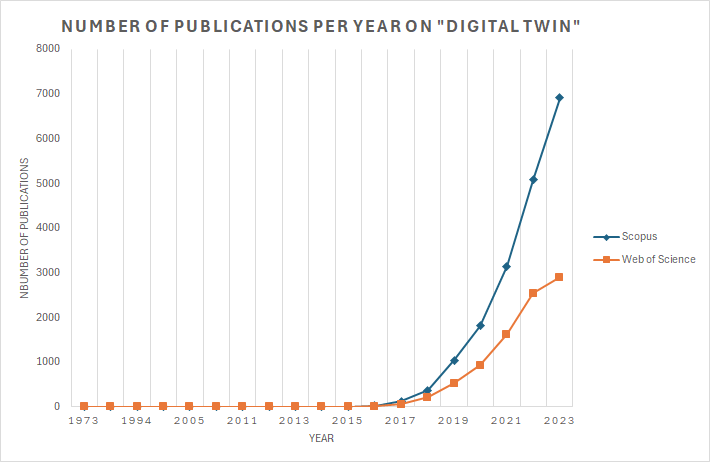
\includegraphics[width=1\linewidth]{resources/number-of-dt-publications-per-year.png}
    \caption{Number of publications per year on "Digital Twin"}
    \label{fig:dt-publications-per-year}
\end{figure}

Figure \ref{fig:dt-publications-per-year} depicts the number of publications per year on Digital twin from two major databases: Web of Science and Scopus. It is evidenced from the graph that research in Digital Twin has witnessed exponential growth in yearly publication in recent years.

It is unclear, however, whether the cloud-native space will adopt Digital Twin at a similar pace in the next years. This is largely due to the fact that the first mention of Digital Twin in cloud-native context was in 2021 for both databases. Hence, there is not enough data to reach a definitive conclusion on the future growth of Digital Twin in cloud-native applications. Still, judging by the available data from 2021 to 2023, the research interests in Digital Twin is rising steadily over the years (Figure \ref{fig:cloud-native-dt-publications}).

\begin{figure}
    \centering
    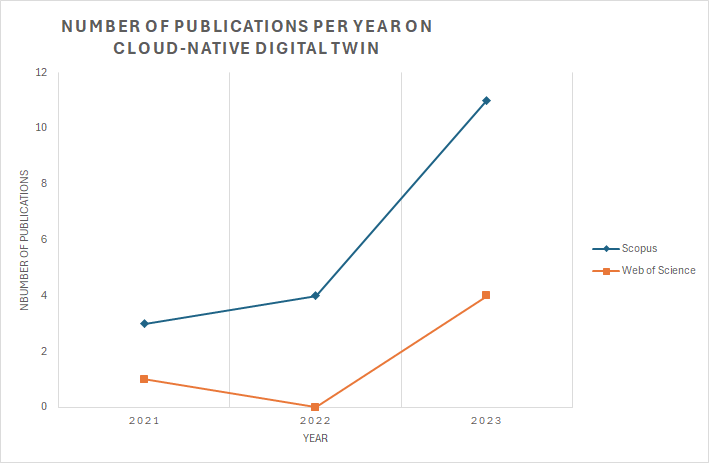
\includegraphics[width=1\linewidth]{resources/cloud-native-dt-publications.png}
    \caption{Number of publications per year on cloud-native digital twin}
    \label{fig:cloud-native-dt-publications}
\end{figure}

\section{Industrial applications and added benefits}

\textit{NOTE:}

- Talk about areas where Digital Twins have been applied, and the benefits provided by said application. Some likely areas to explore are: mining, manufacturing, logistics, and software applications

\section{Digital twin for cloud-native applications}

\textit{NOTE:} This will be the longest section and will contain appropriate subsections as insights arise from the research process \\

\subsection{Cloud-native applications}
\subsubsection{Definition}

\hl{\textit{- TODO: Look into identifying more official standards}}

\par{~}
The Cloud-Native Computing Foundation (CNCF), part of the Linux Foundation, is an organisation that seeks to drive forward the Cloud-native technologies and practices. They are the leading body in terms of setting industrial standards in the Cloud-native space, as was the case for many of the projects that they supported, such as Kubernetes, Prometheus, HELM, and ArgoCD. CNCF defined cloud-native as technologies that enable the development and deployment of scalable applications in cloud environments \cite{cloud_native_computing_foundation_who_nodate}. The application could be hosted on public, private, or hybrid cloud, but in order to support the previously mentioned requirements, they might share the following characteristics:

\begin{enumerate}
\item
  \textbf{Containers}: Compact, self-sufficient units containing all necessary components to run software, promoting uniformity from development through to deployment.
\item
  \textbf{Service Meshes}: Infrastructure layer that facilitates direct and manageable communication within microservices setups, enhancing clarity and control over service interactions.
\item
  \textbf{Microservices}: Design philosophy that organises applications into a network of small, independent services, each fulfilling a specific atomic function.
\item
  \textbf{Immutable Infrastructure}: Method that involves renewing or reconstructing infrastructure elements instead of modifying them, aiming to minimise discrepancies and prevent failures.
\item
  \textbf{Declarative APIs}: Interfaces that enable developers to define their requirements explicitly without detailing the execution process, streamlining application oversight by hiding the complexity of the underlying operations.
\end{enumerate}

\subsection{Historical development}

- Talk about how digital twin has been applied in cloud-native applications (where it started, what were some innovations, and the current state of affairs) \\


- What are some current challenges (problems) in applying digital twins to cloud-native applications, and what are some noteworthy attempts (solutions) to address these challenges \\

\subsection{Added benefits}
\subsubsection{AIOps integration}
\parendline{Self-tuning application}

As previously established, Digital Twin technology allows continuous simulation and monitoring of a given application to gather insights that allow for informed decisions regarding the application's lifecycle. In various applications, these decisions are made by the system administrator or through some pre-defined automation process \cite{jiang_industrial_2021}. While this ability to monitor and predict how the application behaves under certain conditions can be quite powerful, the process still requires human intervention.

In 2022, A. Bhardwa and T. A. Benson have detailed in their paper the potential of integrating AIOps into digital twinning frameworks for application life-cycle management \cite{bhardwaj_kubeklone_2023}.

The proposed framework is called Kubeklone, and it aims to simulate cloud-native applications via digital twinning. An overall architectural view of the framework can be seen in Figure \ref{fig:kubeklone-architecture}. The main difference between AIOps and traditional Digital twin approaches is the introduction of a Machine Learning Playground component to perform analysis on the generated data. Furthermore, this data analysis step and the application configuration step are connected seamlessly. This enables the possibility of having the application tune itself to find the most optimal operation parameters and configurations.

\begin{figure}[h]
    \centering
    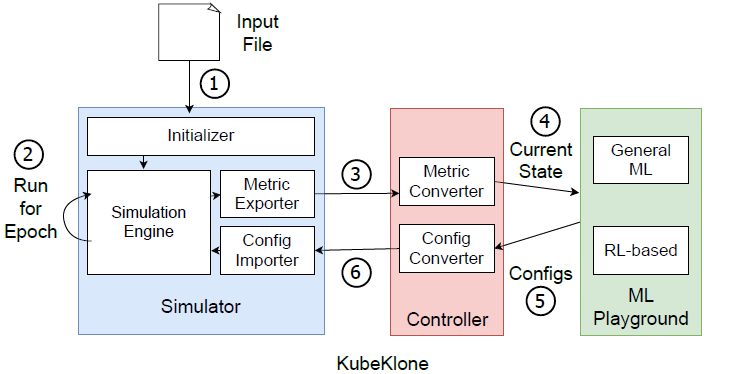
\includegraphics[width=1\linewidth]{resources/kubeklone_architecture.png}
    \caption{Kubeklone's architecture \cite{bhardwaj_kubeklone_2023}}
    \label{fig:kubeklone-architecture}
\end{figure}



\newpage 

\begin{figure}[h]
    \centering
    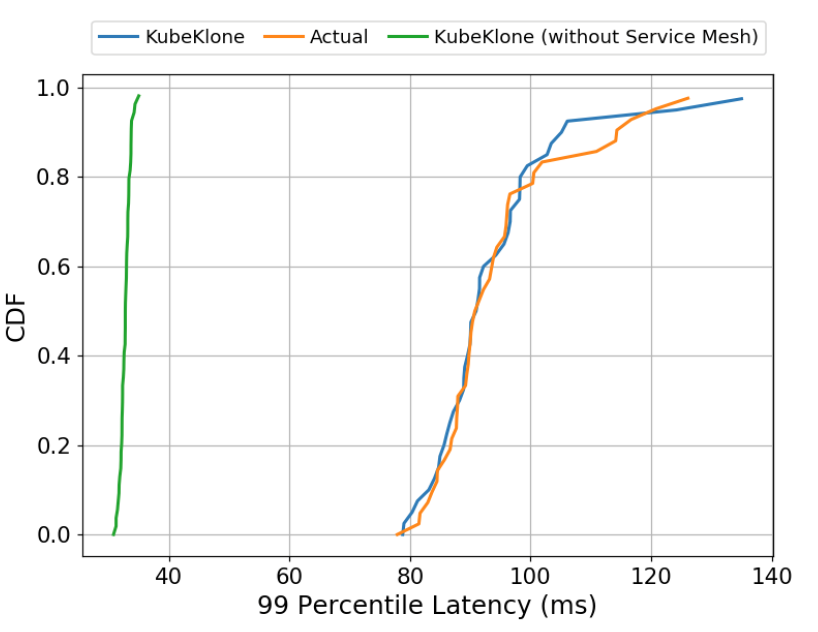
\includegraphics[width=0.7\linewidth]{resources/kubeklone_simulation_results.png}
    \caption{CDF of 99th Percentile Latency for Multiple Runs of the experiment in the (i) Actual Cluster, (ii) KubeKlone, (iii) KubeKlone (without Service Mesh) \cite{bhardwaj_kubeklone_2023}}
    \label{fig:kubeklone-simulation-results}
\end{figure}



The above figure compares the CDF of the latency metric for Kubeklone and that of the Kubernetes cluster it was simulating. The current results are promising, with the simulated Digital Twin mirroring quite closely the performance of the actual Kubernetes cluster.

One aspect worth noting is the available ML Algorithms that the paper demonstrated. The implementation of the ML Playground component supports the use of either (1) General ML (non-Deep Reinforcement Learning algorithms) or (2) Deep Reinforcement Learning. 

Deep RL has witnessed rapid advancements in recent years. An example of this is the breakthrough by NVIDIA researchers in applying generative AI to improve the performance of RL algorithms \cite{ma_eureka_2023}. Eureka, the AI agent in question, was observed to outperform human experts 83\% of the time. As further advancements in Deep RL and other ML algorithms are made, we will likely witness considerable growth in the potential and capabilities of Kubeklone and similar AIOps frameworks.

Despite its potential, Kubeklone as a framework raises some possible concerns regarding the accuracy of its Digital Twinning process. The paper mentioned the abstraction of "all infrastructure components at the request level". In other words, the underlying mechanism of servicing requests for the Microservices within the application architecture is not simulated by Kubeklone. Instead, the developer needs to record the distribution of processing time for all of the services. Kubeklone will then use these distributions to simulate the response time of each microservice (and in turn, the application as a whole).

It is unclear whether this abstraction of the underlying infrastructure components of the application creates any deviation in the Digital Twin's behaviour compared to the real system. In the fidelity validation step, it was mentioned that Kubeklone can replicate the CPU utilisation against the actual deployment rather reliably. However, this only holds for the specified processing time distribution and client request distribution. These distribution curves fail to capture the complex nature of a real application, where various unanticipated failures and stress on the system could happen \cite{basiri_chaos_2016}. Indeed, each failure and stressor introduced to a real-world system might give rise to a completely distinct request processing time distribution.

Due to the abstraction of the mechanism underneath the service layer, Kubeklone, in its current form, lacks the ability to perform planned failure injections. In real systems, corner cases do happen and can lead to catastrophic system failures if not handled correctly \cite{basiri_chaos_2016}. Therefore, failure injection can be a helpful tool for observing the behaviours of the application under harsh conditions and validating its resiliency. 

In addition to the accuracy concern above, the abstraction of the request servicing mechanism created one further step for the developer to "capture a microservice model by running the microservice in a cluster and capturing the request processing times (distribution of processing times) for the different services." This requirement for service processing time is more than just an inconvenience to the developer. The requirement effectively reduces the applicability of Kubeklone for CI/CD pipelines, as human intervention unavoidably interrupts an otherwise automated process. 

Despite the aforementioned shortcomings, simulating microservices through these parameters does make Kubeklone more lightweight than a full DT with all the features of the real system. In addition, since the microservices do not need to run the actual process for request servicing, this effectively unlocks the capability to compress time and run the tuning cycle at a much more rapid pace. This allows Kubeklone to execute the tuning cycle in a much shorter period than a full-fledged digital twin deployment. As similar frameworks to Kubeklone are developed, it would be important to take into consideration this trade-off between accuracy and performance to better serve the particular DT use cases.

\subsubsection{Chaos Engineering}

Chaos Engineering was first coined by a team of researchers from Netflix in a 2016 paper titled with the same term \cite{basiri_chaos_2016}. As briefly mentioned in the section about Kubeklone, Chaos Engineering is the process of injecting planned failure into a given system to test its resiliency in non-optimal conditions.

The paper listed four principles that Chaos Engineering is built upon:

\begin{enumerate}
    \item Building a hypothesis around steady-state behaviour
    \item Vary real-world events
    \item Run experiments in production
    \item Automate experiments to run continuously
\end{enumerate}

In essence, the steady-state behaviour is how the system behaves under normal operating conditions. In Netflix's case, they used the number of streams started per second as the benchmarking metric that defines this steady-state behaviour. This steady state behaviour acts as a reference point to compare observations during Chaos experiments. For instance, if an application was able to maintain its steady state performance even after various chaos injections, we can say with relatively high confidence that the given application is largely resilient to faults.

With a steady state behaviour defined, we can inject certain stimuli into the system based on potential real-world events. The paper stressed that these experiments should be carried out continuously in a production environment to provide up-to-date data that is representative of the system's behaviour.

In this regard, an identical Digital Twin can be used instead of the production system to ensure safety. The paper mentioned the trade-off between the realism of the chaos engineering experiments and the potential risk to the system. This trade-off could be negated by safely performing chaos engineering on a Digital Twin of the application instead of in a production environment.

In addition to ensuring the system's safety, performing chaos engineering on a Digital Twin also increases the capacity for automation. As the authors suggested, letting automation perform Chaos experiments can be potentially risky since these experiments are introducing stimuli that could lead to system failures. This leads to a need for constant monitoring of the automation to ensure that everything is running smoothly. Thus, reducing the degree of automation that the framework can have. Naturally, this risk from automation would be greatly minimised if the experiments are applied to a Digital Twin instead of the production deployment. With the risk of harming the system out of the way, this could unlock a much more comprehensive degree of Chaos experiments, all continuously running alongside the production deployment with absolute safety.

As mentioned in the Background section, research on Digital Twin did not pick up momentum until 2017. Since the Netflix paper was published in 2016, it is reasonable to expect that they did not have the technical knowledge and the architectural support to apply digital twin in the Chaos Engineering experiments. However, due to the benefits above, Chaos Engineering a potential area for Digital Twin application in the future.  


\chapter{Methodology}


\hl{\textit{- TODO: Discuss the overall research design and how the literature review sections relates to the experiment}}    \\
\hl{\textit{- TODO: Discuss the experiment setup for the evaluation of Kubernetes cluster initialization methods, including the tools, environments, and metrics used.}}    \\
\hl{\textit{- TODO: Data collection and analysis}}   \\

\chapter{Experiment}

\hl{\textit{- TODO: Evaluation of cluster provisioning methods}}  \\
\hl{\textit{- TODO: Walk through and compare the results for the tools' metrics}}

\chapter{Discussion}


\hl{\textit{- TODO: Discuss the key findings from the experimentation result (and the literature review if relevant)}}  \\

\chapter{Conclusion}

- Concluding remarks


\chapter*{Acknowledgements}

\par{~}

% I would like to thank my supervisor, Prof. Gopika Premsankar, for her invaluable patience and thorough feedback on the thesis. The research and writing process has been an incredibly fruitful learning experience thanks to her guidance and support.

% This thesis was written with support from Nokia Corporation with regard to the technical details as well as theoretical understanding of the concepts. Major thanks to Mr. Daniel Tyrode---Lead Architect at Nokia's Cloud and Network Services business group---for generously offering his knowledge and expertise as well as constant feedback throughout the process.



%%  LIITTEET  ------------------------------------------

% \appendix
% \chapter{Ut purus elit}

% Lorem ipsum dolor sit amet, consectetuer adipiscing elit. Ut purus
% elit, vestibulum ut, placerat ac, adipiscing vitae, felis. Curabitur
% dictum gravida mauris. Nam arcu libero, nonummy eget, consectetuer id,
% vulputate a, magna. Donec vehicula augue eu neque. Pellentesque
% habitant morbi tristique senectus et netus et malesuada fames ac
% turpis egestas. Mauris ut leo. Cras viverra metus rhoncus sem. Nulla
% et lectus vestibulum urna fringilla ultrices. Phasellus eu tellus sit
% amet tortor gravida placerat. Integer sapien est, iaculis in, pretium
% quis, viverra ac, nunc. Praesent eget sem vel leo ultrices
% bibendum. Aenean faucibus. Morbi dolor nulla, malesuada eu, pulvinar
% at, mollis ac, nulla. Curabitur auctor semper nulla.  Donec varius
% orci eget risus. Duis nibh mi, congue eu, accumsan eleifend, sagittis
% quis, diam. Duis eget orci sit amet orci dignissim rutrum.

% Nam dui ligula, fringilla a, euismod sodales, sollicitudin vel,
% wisi. Morbi auctor lorem non justo. Nam lacus libero, pretium at,
% lobortis vitae, ultricies et, tellus. Donec aliquet, tortor sed
% accumsan bibendum, erat ligula aliquet magna, vitae ornare odio metus
% a mi. Morbi ac orci et nisl hendrerit mollis. Suspendisse ut
% massa. Cras nec ante. Pellentesque a nulla.  Cum sociis natoque
% penatibus et magnis dis parturient montes, nascetur ridiculus
% mus. Aliquam tincidunt urna. Nulla ullamcorper vestibulum
% turpis. Pellentesque cursus luctus mauris.

% \section{Fusce mauris}

% Fusce mauris. Vestibulum luctus nibh at lectus. Sed bibendum, nulla a
% faucibus semper, leo velit ultricies tellus, ac venenatis arcu wisi
% vel nisl.  Vestibulum diam. Aliquam pellentesque, augue quis sagittis
% posuere, turpis lacus congue quam, in hendrerit risus eros eget
% felis. Maecenas eget erat in sapien mattis porttitor. Vestibulum
% porttitor. Nulla facilisi.  Sed a turpis eu lacus commodo
% facilisis. Morbi fringilla, wisi in dignissim interdum, justo lectus
% sagittis dui, et vehicula libero dui cursus dui. Mauris tempor ligula
% sed lacus. Duis cursus enim ut augue. Cras ac magna.  Cras
% nulla. Nulla egestas. Curabitur a leo. Quisque egestas wisi eget
% nunc. Nam feugiat lacus vel est. Curabitur consectetuer.

\renewcommand{\bibname}{References (IEEE style)}
\bibliography{references.bib}

\end{document}